\documentclass[a4paper,12pt,oneside,openany,table,xcdraw]{article}

\usepackage{setspace}
\usepackage{multirow}
\usepackage{hyperref}
\usepackage{caption}
\usepackage{indentfirst}

\usepackage[brazilian]{babel}
\usepackage[utf8x]{inputenc}
\usepackage{amsmath, graphicx, mathptmx, enumerate}
\usepackage{float, verbatim}
\usepackage[colorinlistoftodos]{todonotes}
\usepackage{makeidx} % Para o sumário
\usepackage{geometry}

\geometry{a4paper, hmargin={3cm, 3cm}, vmargin={3cm, 2cm} }
\setlength{\parindent}{1.0cm}

\begin{document}
\newcommand{\thedepartment}{Faculdade de Engenharia Elétrica}
\newcommand{\thecourse}{FEELT}
\newcommand{\thetitle}{CIRCUITOS ACOPLADOS MAGNETICAMENTE}
\newcommand{\thetype}{Relatório da Disciplina de Circuitos Elétricos II}
\newcommand{\theproftitle}{Bacharel em Engenharia Elétrica}
\newcommand{\thestudent}{Lesly Viviane Montúfar Berrios\\
\centering11811ETE001}
\newcommand{\theadvisor}{Prof. Wellington Maycon Santos Bernardes}
\newcommand{\thecity}{Uberlândia}

\thispagestyle{empty}\newcommand*{\themonth}{\ifthenelse{\the\month < 2}{Janeiro }
                  {\ifthenelse{\the\month < 3}{Fevereiro }
                  {\ifthenelse{\the\month < 4}{Março }
                  {\ifthenelse{\the\month < 5}{Abril }
                  {\ifthenelse{\the\month < 6}{Maio }
                  {\ifthenelse{\the\month < 7}{Junho }
                  {\ifthenelse{\the\month < 8}{Julho }
                  {\ifthenelse{\the\month < 9}{Agosto }
                  {\ifthenelse{\the\month < 10}{Setembro }
                  {\ifthenelse{\the\month < 11}{Outubro }
                  {\ifthenelse{\the\month < 12}{Novembro }{Dezembro }}}}}}}}}}}}
                  
\begin{titlepage}
\begin{center}

	\vspace{-0.5cm}

  \begin{figure}[hbt!]
		\begin{center}
		   
\includegraphics[width=2.8cm]{ufu-logo.png}
		\end{center}
	\end{figure}
 	%\vspace{-4cm}

%\begin{doublespacing}

  \Large{\textbf{Universidade Federal de Uberlândia}}\\
  \large{\thedepartment}\\
  \large{\thecourse}\\


\vspace{5.8cm}
  \par
  \large\textbf{\thetitle}
\vspace{5.8cm} 

%\end{doublespacing}
  \par
  \thetype\\
  por\\
  %\hspace{2cm}\large{}\\

\vspace{0.8cm}
\par
  \normalsize{\thestudent}\\ [2cm]
  \theadvisor

\par\vfill
  \thecity, \themonth / \the\year

\end{center}

\end{titlepage}

%% Comeca o documento !

\onehalfspacing
\tableofcontents % sumário
\newpage

\section{Objetivos} % 2,5%
Verificar experimentalmente os conceitos teóricos sobre acoplamentos magnéticos,
obtenção dos valores das auto-indutâncias e da indutância mútua, e comparar os resultados
com os valores obtidos utilizando uma análise teórica.

\section{Introdução teórica} % 5%
Nos circuitos em que a condução de energia elétrica ocorre por meios físicos, diz-se que são circuitos condutivos. Entretanto, ainda é possível que dois circuitos com ou sem contato se afetem por meio do campo magnético gerado por um deles, esses são chamados circuitos magneticamente acoplados \cite{ph}.

O \emph{transformador} é baseado nesse princípio. Possui quatro terminais e consiste em dois indutores que são colocados com certa proximidade um do outro, logo comparttilham o mesmo fluxo magnético e, portanto, as bobinas indutoras estão acopladas magneticamente. 

Sua aplicabilidade é vasta, por exemplo, em sistemas de comunicação, são usados para casamento de impedâncias entre fontes e cargas ou linhas de transmissão. Em sistemas de potências, transformadores são usados para atenuar ou amplificar os sinais de tensão. De fato, transformadores são utilizados em eliminadores de pilha e recarregadores de baterias, que podem ser ligados diretamente em tomadas residenciais \cite{irwin}.

\subsection{A Indutância Mútua}
 Enrolamentos acoplados magneticamente dão origem ao fenômeno de indutância mútua. Os indutores podem neste experimento são acoplados em série, o que permite o cálculo da indutância mútua a partir da Equação (\ref{mutua}), considerando a natureza não-ideal dos transformadores.

Da ligação série aditiva e subtrativa tem-se os resultados das Equações (\ref{ad}) e (\ref{sub}) para os módulos das impedâncias obtidas.
\begin{equation}\label{ad}
Z_{ad}^2=(R_1+R_2)^2+(\omega L_1+\omega L_2+\omega2M)^2
\end{equation}
\begin{equation}\label{sub}
Z_{sub}^2=(R_1+R_2)^2+(\omega L_1+\omega L_2-\omega2M)^2
\end{equation}

Assim, tem-se:
\begin{equation}
L_1+L_2=\dfrac{\sqrt{Z_{ad}^2-(R_1+R_2)^2}-2\omega M}{\omega}
\end{equation}
\begin{equation}
L_1+L_2=\dfrac{\sqrt{Z_{sub}^2-(R_1+R_2)^2}+2\omega M}{\omega}
\end{equation}
\vspace{0.1cm}

Portanto, a indutância mútua será dada por:
\begin{equation}\label{mutua}
M = \dfrac{1}{4\omega}\ \bigg(\sqrt{Z_{add}^2-(R_1+R_2)^2} - \sqrt{Z_{sub}^2-(R_1+R_2)^2}\bigg)
\end{equation}
\vspace{0.01cm}

A indutância mútua surge devido a interação do fluxo magnético do primário ($\phi_p$) nos terminais do secundário, o que provoca uma tensão induzida. Entretanto, para transformadores não-ideais somente uma parcela do fluxo que percorre o primário também percorre o secundário ($\phi_m$). Assim, é interessante definir o \textbf{coeficiente de acoplamento} $k$ entre os dois enrolamentos, descrito pela Equação (\ref{k}).

\begin{equation}\label{k}
k = \dfrac{\phi_m}{\phi_p}
\end{equation}

\subsection{Cálculo das indutâncias próprias}
Para o cálculo das impedâncias próprias é analisado o experimentalmente um transformador a vazio

\section{Preparação}
\subsection{Materiais e ferramentas} % 2,5%
\begin{enumerate}[1 - ]
\item \emph{Fonte}\\
Alimentará todo o circuito.

\item \emph{Conjunto de bobinas}\\
Cada bobina possui uma resistência, sendo $R_1$ para a bobina 1 e $R_2$ para a bobina 2. Considere $R_1<R_2$.

\item \emph{Conectores}\\
Foram utilizadas pontas de provas para a verificação das grandezas nos multímetros. Para as conexões no circuito foi utilizado majoritariamente cabos banana-banana.

\item \emph{Multímetro}\\
Utilizado para medir as tensões elétricas entre os pontos das bobinas especificados no experimento.

\item \emph{Miliamperímetro}\\
A escala mais precisa permite melhor regulagem da corrente desejada.

\item \emph{Varivolt}\\
O equipamento permitirá obter o valor desejado de corrente a partir da regulagem correta da tensão fornecida pela fonte.


\end{enumerate}

\subsection{Montagem} % 2,5%
\begin{enumerate}[1)]
\item \emph{Resistências das bobinas}\\
Para o conjunto de bobinas fornecido, foi medido a resistência da bobina 1 (600 esp.) e a
resistência da bobina 2 (1200 esp.) e obteve-se: 
$$R_1= 2,6\Omega$$ $$R_2=7,4\Omega$$

\item \emph{Determinando a polaridade das bobinas}\\
Efetue a montagem da Figura \ref{2.2}, aplicando uma corrente de 50 mA no
miliamperímetro, anote a tensão $V_1$ e marque a
polaridade da Bobina 1, indicando-a por um ponto “.”, no terminal em que a fem1 (terminal
ligado ao positivo da fonte CA) é positiva. Na bobina 2 marque a polaridade (o ponto) no
terminal ligado ao voltímetro se a tensão $V’< V1$, e marque o ponto no
terminal debaixo se $V’>V_1$ (terminal em que a fem induzida é positiva). 

\begin{figure}[h]
\centering
\captionsetup{font=scriptsize}
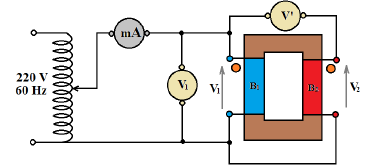
\includegraphics[width=11cm]{fig1}
\caption{Marcação de polaridade.}
\label{2.2}
\end{figure}

Da análise experimental, obteve-se $V'=8,33V$ e $V_1=10,27V$. Logo, o ponto é indicado como na Figura \ref{2.2}, ponto no terminal superior da bobina 2, pois $V’< V1$.

\item \emph{Ligação série aditiva}\\
Como na Figura \ref{2.3}, a montagem faz a ligação em série aditiva das bobinas 1 e 2 (os fluxos são aditivos). Aplique a tensão necessária de modo a obter o valor de corrente
indicado na Tabela \ref{tab1}, completando as demais colunas com os valores das tensões V (tensão
total aplicada as bobinas). Os valores de $Z_{ad}$ são obtidos fazendo $V/I$.

\begin{figure}[h]
\centering
\captionsetup{font=scriptsize}
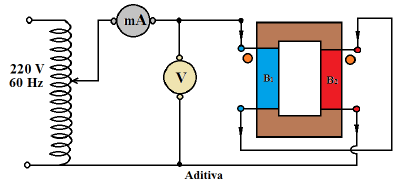
\includegraphics[width=11cm]{fig2}
\caption{Ligação série aditiva das bobinas 1 e 2}
\label{2.3}
\end{figure}
\begin{table}[H]
\centering
\def\arraystretch{1.35}
\captionsetup{type=table, font=scriptsize}
\caption{Tabela de tensões para cada valor de corrente $I_{ad}$ setado.} \label{tab1}
\begin{tabular}{|c|c|c|}
\hline
$I_{ad}$ (mA) & V (V) & $Z_{ad} (\Omega)$ \\ \hline
16,7        & 32,66 & 1955,68            \\ \hline
33,3        & 61,55 & 1848,34            \\ \hline
50,0        & 94,60 & 1892,00            \\ \hline
\end{tabular}
\end{table}

\item \emph{Ligação série subtrativa}\\
Como na Figura \ref{2.4}, a montagem faz a ligação em série subtrativa entre as bobinas 1 e 2 (fluxos subtrativos ou
contrários). Aplique a tensão necessária de modo a obter as correntes indicadas na Tabela \ref{tab2}, completando as demais colunas com os valores das tensões V (tensão
total aplicada as bobinas). Os valores de $Z_{sub}$ são obtidos fazendo $V/I$.

\begin{figure}[h]
\centering
\def\arraystretch{1.35}
\captionsetup{font=scriptsize}
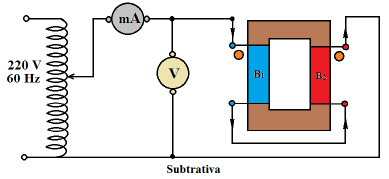
\includegraphics[width=11cm]{fig3}
\caption{Ligação série subtrativa das bobinas 1 e 2.}
\label{2.4}
\end{figure}
\begin{table}[h]
\centering
\def\arraystretch{1.35}
\captionsetup{type=table, font=scriptsize}
\caption{Tabela de tensões para cada valor de corrente $I_{sub}$ setado.} \label{tab2}
\begin{tabular}{|c|c|c|} 
\hline
$I_{sub}$ (mA) & V (V) & $Z_{sub} (\Omega)$ \\ \hline
50,0          & 15,20 &  304,00           \\ \hline
100,0        & 31,11 & 311,10            \\ \hline
150,0        &46,09  & 307,27            \\ \hline
\end{tabular}
\end{table}


\item \emph{Transformador a vazio}\\
Efetue a montagem do circuito da Figura \ref{2.5} abaixo, considerando agora as bobinas 1 e 2
isoladas (como num transformador a vazio). Aplique uma tensão na bobina 1 de modo a
obter a corrente indicada na Tabela \ref{tab3}. Meça a tensão na bobina 1 ($V_1$) e a tensão que é
induzida na bobina 2 devido a corrente na bobina 1 ($V_2$). Os valores de $Z_1$ são obtidos fazendo $V/I$.

\begin{figure}[h]
\centering
\captionsetup{font=scriptsize}
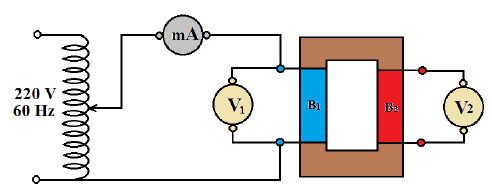
\includegraphics[width=11cm]{fig4}
\caption{Transformador com bobina 1 no primário e bobina 2 no secundário.}
\label{2.5}
\end{figure}
\begin{table}[h]
\centering
\def\arraystretch{1.35}
\captionsetup{type=table, font=scriptsize}
\caption{Tabela de tensões para cada valor de corrente $I_1$ setado} \label{tab3}
\begin{tabular}{|c|c|c|c|}
\hline
$I_1$ (mA) & $V_1$ (V)  & $Z_{1} (\Omega)$ & $V_2$ (V) \\ \hline
50,0          & 10,30  &  206,00       &  18,61     \\ \hline
100,0        & 21,14  &  211,40       &  38,44   \\ \hline
150,0        & 32,14  &  214,27       &  59,01   \\ \hline
\end{tabular}
\end{table}

\item \emph{Transformador a vazio com bobinas invertidas}\\
Efetue a montagem do circuito da Figura \ref{2.6} abaixo, considerando agora as bobinas 1 e 2
isoladas (como num transformador a vazio). Aplique uma tensão na bobina 2 de modo a
obter a corrente indicada na Tabela \ref{tab4}. Meça a tensão na bobina 1 ($V_1$) e a tensão que é
induzida na bobina 2 devido a corrente na bobina 1 ($V_2$). Os valores de $Z_1$ são obtidos fazendo $V/I$.

\begin{figure}[h]
\centering
\captionsetup{font=scriptsize}
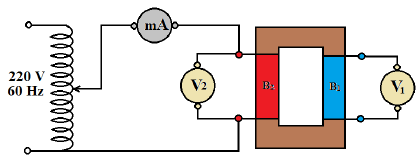
\includegraphics[width=11cm]{fig5}
\caption{Transformador com bobina 2 no primário e bobina 1 no secundário}
\label{2.6}
\end{figure}
\begin{table}[h]
\centering
\def\arraystretch{1.35}
\captionsetup{type=table, font=scriptsize}
\caption{Tabela de tensões para cada valor de corrente $I_1$ setado} \label{tab4}
\begin{tabular}{|c|c|c|c|}
\hline
$I_2$ (mA) & $V_2$ (V)  & $Z_{2} (\Omega)$ & $V_1$ (V) \\ \hline
25,0          & 20,97  &  838,80       &  9,81     \\ \hline
50,0          & 43,53  &  870,60       &  19,14   \\ \hline
75,0          & 66,30  &  884,00       &  29,43   \\ \hline
\end{tabular}
\end{table}

\end{enumerate}

\section{Análise sobre segurança} % 2,5%
Os óculos de segurança são Equipamentos de Proteção Individual (EPIs) e são utilizados para a proteção da área ao redor dos olhos contra qualquer tipo de detrito estranho, que possa causar irritação ou ferimentos. Também protegem contra faíscas, respingos de produtos químicos, detritos, poeira, radiação e etc \cite{safe}.
É importante a utilização desse equipamento durante os experimentos a fim de evitar qualquer dano, além de preparar o profissional para o manejo correto e seguro de qualquer equipamento.

\section{Cálculos, análise dos resultados e questões} %(quando houver) (70%)

\begin{enumerate}[1 - ]
\item A partir dos valores obtidos na tabela \ref{tab1}, encontre o valor médio da impedância $Z_{ad}$.\\
O valor médio da impedância $Z_{ad}$ será:
$$Z_{ad}=1898,67\Omega$$

\item A partir dos valores obtidos na tabela \ref{tab2}, encontre o valor médio da impedância $Z_{sub}$.
Com os valores médios das impedâncias aditiva e subtrativa e os valores das resistências das
bobinas ($R_1$ e $R_2$), encontre o valor da impedância mútua $M$. \\
O valor médio da impedância $Z_{sub}$ será:
$$Z_{sub}=307,42\Omega$$

Assim, a indutância mútua será dada por meio da Equação (\ref{mutua}).
\begin{equation*}
M = \dfrac{1}{4\times(2\pi \cdot 60)}\ \bigg(\sqrt{1898,67^2-(2,6+7,4)^2} - \sqrt{307,42^2-(2,6+7,4)^2}\bigg) = 1,0553 H
\end{equation*}


\item A partir dos valores obtidos na tabela \ref{tab3}, encontre o valor médio da impedância $Z_1$.\\
O valor médio da impedância $Z_{1}$ será:
$$Z_{1}=210,56\Omega$$

\item A partir dos valores obtidos na tabela \ref{tab4}, encontre o valor médio da impedância $Z_2$.
Com os valores médios das impedâncias das bobinas ($Z_1$ e $Z_2$) e os valores das resistências
das bobinas ($R_1$ e $R_2$), encontre os valores das reatâncias próprias e das auto indutâncias $L_1$
e $L_2$.\\
O valor médio da impedância $Z_{2}$ será:
$$Z_{2}=864,47\Omega$$



\item Com os valores obtidos para $L_1$, $L_2$ e $M$ encontre o valor do coeficiente de acoplamento
entre as bobinas 1 e 2. \\
A partir equação

\item Para uma corrente de $1,0 A$ na bobina 1 (Figura \ref{2.5}), encontre o valor do fluxo $\phi_1$, $\phi_{L1}$. \\
\item Para uma corrente de $1,0 A$ na bobina 1 (Figura \ref{2.6}), encontre o valor do fluxo $\phi_2$, $\phi_{L2}$. \\

\item O que deve acontecer com as leituras dos instrumentos do primário, em qualquer das
montagens efetuadas, se a barra superior do núcleo de ferro for removida (o núcleo for
aberto)? \\

\item O que deve acontecer com as leituras dos instrumentos do secundário, em qualquer das
montagens efetuadas, se o núcleo de ferro for retirado do circuito sem desligamento do
mesmo? \\


\end{enumerate}


\section{Simulação computacional} %(10%);

\section{Conclusões} % (no mínimo 10 linhas) (5%)


\newpage
\begin{thebibliography}{9} 
% Introdução
\bibitem{ph}
    P. H. Rezende,
    “Circuitos Magneticamente Acoplados”, UFU, 2018.
 Disponível em:
 \url{https://www.moodle.ufu.br/pluginfile.php/702496/mod_resource/content/3/Cap.\%20I_Acoplamento.pdf}. Acesso em: ago. 2019.

\bibitem{irwin}
    J. D. Irwin,
    “Análise de Circuitos Em Engenharia”, Pearson, $4^a$ Ed., 2000.

\bibitem{boylestad}
    R. L. Boylestad,
    “Intrdução À Análise de Circuitos”, Pearson, $10^a$ Ed., 2004.


\bibitem{safe}
    SafetyTrabi,
    “Óculos de segurança: Saiba quando utilizar este EPI”, SafetyTrab, 2019.
 Disponível em:
 \url{https://www.safetytrab.com.br/blog/oculos-de-seguranca/}. Acesso em: ago. 2019.




\end{thebibliography}
\end{document}